\documentclass[letterpaper,12pt]{article}
\usepackage[utf8]{inputenc}

\usepackage[T1]{fontenc}
\usepackage{tgtermes} %%%font


\usepackage[spanish]{babel}

\usepackage{geometry}
\usepackage{amsmath}
\usepackage{float}
\usepackage{graphicx}
\usepackage{subcaption}
\usepackage{amssymb}
\usepackage{adjustbox}
\usepackage{wrapfig} %%imagen envuelta por un texto
\usepackage{xcolor}
\usepackage{fancyhdr}
\usepackage{tabularx} %%TABLAS OH YEAH

\title {\textbf{Conceptos básicos de Administración y Administrador}}
\author{Lara Xocuis Martha Denisse}
\date{1 de septiembre de 2023}
\geometry{top=2cm, bottom=2cm, left=2cm, right= 2cm} %%margen
\graphicspath{{images/}}
\parindent=0pt

\begin{document}
\maketitle

%%%%%%%%%%%%%%%%%%%%%%%%%%%%%%%%%%%%%%%%%%%%%%%%%%%%%%%%%%%%%%%%%%%%%%%%%%%%
\begin{sloppypar}
\section{Definición de Administración}
La administración es una disciplina muy general, algunos autores plantean que es una ciencia, otros que es un arte, lo cierto que esta área ofrece tanto de lo uno como de lo otro y no se le ha prestado la debida atención siendo una herramienta indispensable para desarrollar todas las actividades. 
\vspace{0.3cm}\\
Para interpretar las administración se pueden tomar algunas definiciones ya planteadas: 

\textit{"El proceso de realizar actividades y terminarlas eficientemente con y a través de las personas" (Robbins, 1996, p.5)}
\vspace{0.3cm}\\ 
Una definición más técnica es la planteada por Stoner: \textit{"La administración es el proceso de planear, organizar, dirigir y controlar los esfuerzos de los miembros de la organización, y de aplicar los demás recursos de ella para alcanzar las metas
establecidas."}
\vspace{0.3cm}\\ 
Las definiciones anteriores tienen en común dos cosas, que la administración es un conjunto de funciones y se orienta a un
objetivo específico. La administración se puede definir entonces como el proceso de: \textbf{planear, organizar, dirigir y controlar} para cumplir con el propósito de la organización. De igual forma, si buscamos conceptos básicos en todas las definiciones que podamos revisar, en general se notará que involucran acciones que: 
\begin{itemize}
    \item Requieren el esfuerzo de \textbf{personas}
    \item Necesitan ciertos \textbf{recursos} para poder funcionar 
    \item Tienen que estar orientadas hacia un \textbf{objetivo}
\end{itemize}

\section{¿Por qué es un proceso?}
Si asumimos que la administración involucra acciones que deben ser desempeñadas, se vuelve necesario clasificar dichas acciones para poder entender su funcionamiento. De acuerdo con la mayoría de autores, la Administración tiene cuatro grandes funciones que, relacionadas, forman el llamado \textbf{Proceso Administrativo}
\newpage
\section{Fases}
\begin{itemize}
    \item Planificar: son las acciones necesarias para identificar el objetivo al que se desea llegar, así como el camino para elegir el mismo. Se entiende como la determinación del trabajo que se va a realizar, la proyección de las acciones que se van a desarrollar, así como, el establecimiento de metas y objetivos para la organización y la forma como se van a integrar en el trabajo. 
    \item Organizar : una vez definido el objetivo, es hora de dar un orden interno a los recursos(incluyendo las personas) a fin de que puedan ser utilizados de la mejor manera para alcanzar el objetivo. Es conocido como la organización, la clasificación y división del trabajo en unidades más pequeñas, la coordinación de los recursos de la organización (humanos, técnicas, físicos, entre otros). Además determinar que se necesita hacer, cómo, quien, cuando y donde lo va a realizar.
    \item Dirigir : con un  objetivo claro y recursos alineados, llega el momento de hacer que las personas, a través de sus capacidades y su trabajo, realicen las acciones necesarias para llegar al objetivo, influyendo en los trabajadores para desarrollar las actividades, tomando la responsabilidad sobre el comportamiento humano necesario para cumplir con las metas, ejerciendo un liderazgo sobre el personal de la organización y motivándolo a cumplir con las labores asignadas. 
    \item Controlar : A lo largo del camino que se está siguiendo, se debe verificar que no se esté desviando del objetivo propuesto y, si es así, se deben proponer las medidas correctivas del caso. Se debe de asegurar el cumplimiento de los objetivos, verificando que la organización está en la dirección correcta en la obtención de sus metas. Es el seguimiento de actividades para asegurarse de que el plan se ejecute correctamente. 
\end{itemize}
\section{Definición de Organigrama}
En toda organización es necesario conocer las relaciones que existen entre los elementos que la conforman, así mismo como las posiciones y funciones que realiza cada uno de estos, es necesario entender la estructura interna en general de  la organización; la estructura  es uno de los factores claves para alentar al recurso humano a la competitividad y productividad dando como resultado que la organización logre con éxito sus objetivos.

Teniendo en cuenta, que el organigrama es una representación gráfica que expresa la estructura  jerárquica e interrelación de las distintas áreas o elementos que componen una organización, resulta necesario que todos los que forman parte de dicha organización, conozcan cuál es su definición, para que de esa manera, tengan un conocimiento básico, acerca de lo que es este sencillo pero valioso recurso administrativo.

Existen diferentes definiciones de organigrama algunas de estas son:
\begin{itemize}
    \item Según Ferrel, Hirt, Adriaenséns, Flores y Ramos, autores del libro «Introducción a los Negocios en un Mundo Cambiante», el organigrama es una «representación visual de la estructura organizacional, líneas de autoridad, (cadena de mando), relaciones de personal, comités permanentes y líneas de comunicación”.
    \item Para Enrique B. Franklin, autor del libro «Organización de Empresas», el organigrama es  «la representación gráfica de la estructura orgánica de una institución o de una de sus áreas, en la que se muestran las relaciones que guardan entre sí los órganos que la componen”.
    \item Benjamín Franklin: Un organigrama es la representación gráfica de la estructura orgánica de una institución o de una de sus áreas o unidades administrativas, en las que se muestran las relaciones que guardan entre sí los órganos que la componen.
\end{itemize}

Podemos concluir que: \textbf{El organigrama es la representación gráfica y esquemática de la estructura organizacional en la que se muestran las relaciones que guardan entre si los órganos que la componen.}
\vspace{0.3cm}\\
La finalidad del organigrama es proporcionar información por medio de representaciones gráficas de los aspectos fundamentales de los cuales se conforma la estructura organizacional, permitiendo entender en lo general la relación e integración de los elementos que la conforman. Los organigramas se pueden clasificar por su objetivo que pueden ser funcionales o estructurales, por el área, que pueden ser generales o departamentales y por su conocimiento los cuales pueden ser esquemáticos o analíticos.
\vspace{0.3cm}\\
Por lo regular se diseñan de arriba hacia abajo, mostrando la jerarquía de mayor a menor. El organigrama se compone de rectángulos y cuadros que se unen por medio de líneas, las cuales representan los canales de dependencia y responsabilidades de la institución.

\begin{figure}[H]
    \centering 
    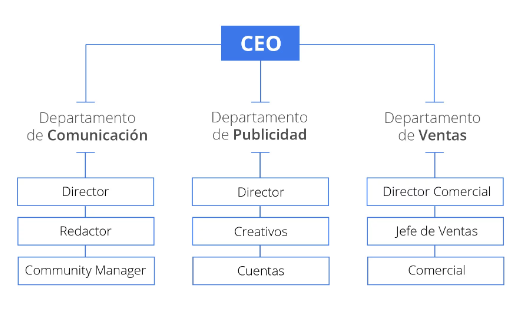
\includegraphics[width=0.7\textwidth]{images/organigrama.png}
    \caption{Ejemplo de un organigrama}
\end{figure}

\section{¿Dónde se ubica el Administrador en el Organigrama?}
En la actualidad, los diversos nombres que se utilizan para los administradores son muchos, gerentes, directores, jefes, entre otros y en general \textbf{se les puede clasificar en tres niveles:} En primer lugar se encuentran los de \textbf{primera línea}, llamados también supervisores responsables de dirigir a los operarios en sus actividades cotidianas, es decir son las personas que están en permanente contacto con los trabajadores y quienes conocen el funcionamiento operativo de la compañía.
\vspace{0.3cm}\\
Luego se encuentran los de \textbf{nivel intermedio}, conocidos como: mandos medios, jefes de departamento o dependencia, líder de proyectos, jefe de unidad, administrador de distrito, decano, obispo o gerente de división. Estos gerentes están encargados de una de las funciones mas complicadas, dirigir a otros administradores (primera línea) o colegas y son responsables de traducir las metas de la organización en objetivos específicos que otros administradores puedan realizar.
\vspace{0.3cm}\\
En el nivel superior o punto más alto de la organización, se encuentra la \textbf{alta gerencia}, la cual tiene nombres como: Presidentes, vicepresidentes, canciller, director general, director o presidente del consejo. La función principal de este nivel es establecer el rumbo que debe tomar la organización.
\vspace{0.3cm}\\
En la siguiente imagen se plantea un ejemplo de los diferentes niveles de una compañía de construcción: los trabajadores se
encuentran por fuera de la administración de la organización y son quienes ejecutan la labor, luego se encuentra el primer nivel de dirección, generalmente profesionales egresados recientemente, luego están sus colegas, los cuales tienen más experiencia que los anteriores y probablemente tienen formación avanzada o alguna especialización y en la cima de la compañía están los profesionales de mayor trayectoria dentro de la organización, las personas que seguramente la crearon y su experiencia hace que estén definiendo el horizonte de la compañía, puede ser el dueño, el gerente
general, administrador o el presidente

\begin{figure}[H]
    \centering
    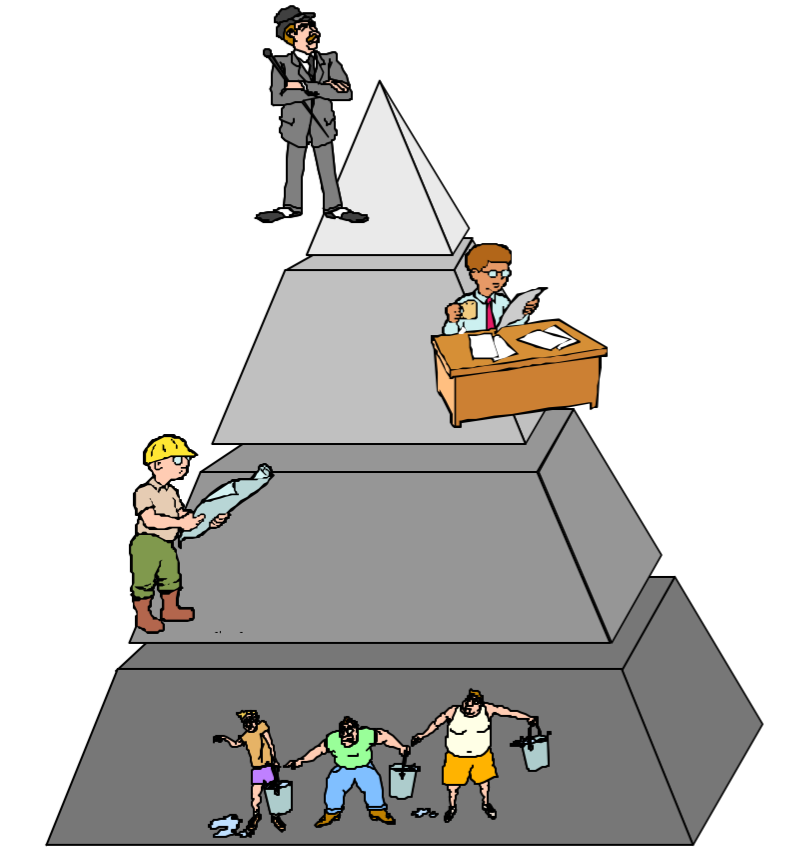
\includegraphics[width=0.4\textwidth]{images/admin.png}
    \caption{Ejemplo de niveles de trabajo dentro de una compañia}
    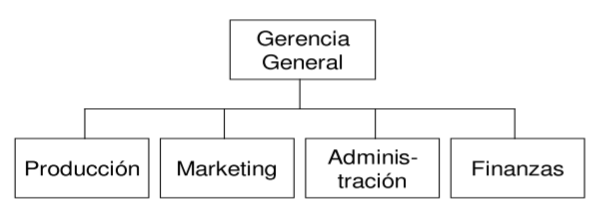
\includegraphics[width=0.7\textwidth]{images/admin2.png}
    \caption{Ejemplo de organigrama empresarial general}
\end{figure}
\newpage
\section{Habilidades y Competencias de un Administrador}
El \textbf{Administrador} debe tener la habilidad gerencial de comprender primero y luego ser comprendido, creando relaciones humanas afectivas que tiendan al ganar–ganar. El trabajo de un administrador se basa en la planeación, organización, integración y la medición.

Los gerentes actuales les gusta lo que hacen, sienten empatía con los demás, cada vez se preparan de mejor manera para desarrollar las capacidades necesarias para tener un buen liderazgo frente a sus equipos de trabajo, administrar con empatía, tomar decisiones acertadas, resolver con éxito los problemas y conflictos, capacidad para trabajar en equipo, saber correr riesgos, innovar, crear, empatizar con las demás personas, entre otros factores que hacen posible el logro de metas y objetivos esperados por la organización basados en la misión y visión. 
\vspace{0.3cm}\\ 
Deben desarrollar habilidades, disciplinas y conocimientos que les permitan llevar a sus equipos de trabajo a la cima, posicionándose en los principales lugares con calidad, logrando los resultados que la organización requiere y un verdadero cambio organizacional. 

\section{Bibliografía}
\textit{Cruz Brambila Gerardo. (2012, junio 8). <em>Organigramas. Definiciones y herramientas</em>. Recuperado de https://www.gestiopolis.com/}
\vspace{0.3cm}\\ 
\textit{FUNDAMENTOS DE ADMINISTRACIÓN PARA INGENIEROS. (Medellín, Enero 2022) Miguel David Rojas López, Marisol Ricaurte Yepes}
\vspace{0.3cm}\\ 
\textit{Fundamentos de Gestión Empresarial. Cibertec}        

\end{sloppypar}
\end{document}